% \documentclass[handout]{beamer}
\documentclass{beamer}

%%
%%
%%
% From http://tex.stackexchange.com/questions/2072/beamer-navigation-circles-without-subsections
% Solution #2 or 3:
% \usepackage{etoolbox}
% \makeatletter
% % replace the subsection number test with a test that always returns true
% \patchcmd{\slideentry}{\ifnum#2>0}{\ifnum2>0}{}{\@error{unable to patch}}%
% \makeatother
% Solution #1:
\usepackage{remreset}% tiny package containing just the \@removefromreset command
\makeatletter
%\@removefromreset{subsection}{section}
%\makeatother
%\setcounter{subsection}{1}




\usepackage{etex}
\usepackage{pgf}
\usepackage{tikz}
\usepackage{url}
\usepackage{amsmath}
\usepackage{color}
% \definecolor{red}{rgb}{1,0,0}
\usepackage{ulem}
% \usepackage{booktabs}
\usepackage{colortbl,booktabs}
\renewcommand*{\thefootnote}{\fnsymbol{footnote}}
\usepackage{fancybox}
\usepackage[framemethod=TikZ]{mdframed}
\mdfdefinestyle{FactStyle}{%
  outerlinewidth=0.5,
  roundcorner=1pt,
  leftmargin=1cm,
  linecolor=blue,
  outerlinecolor=blue!70!black,
  backgroundcolor=yellow!40
}
\usepackage{cancel}

  \newcommand\Warning{%
    \makebox[2.4em][c]{%
      \makebox[0pt][c]{\raisebox{.2em}{\Large!}}%
      \makebox[0pt][c]{\color{red}\Huge$\bigtriangleup$}}}%

\usepackage{stackengine}
\usepackage{scalerel}
\usepackage{xcolor}
  \newcommand\dangersign[1][2ex]{%
    \renewcommand\stacktype{L}%
    \scaleto{\stackon[1.3pt]{\color{red}$\triangle$}{\tiny !}}{#1}%
  }



\usepackage{dcolumn}
\newcolumntype{d}[1]{D{.}{.}{#1}}

% From
% http://tex.stackexchange.com/questions/109900/how-can-i-box-multiple-aligned-equations
\usepackage{empheq}
\usepackage{tcolorbox}  \newtcbox{\othermathbox}[1][]{%
  nobeforeafter, tcbox raise base, 
  colback=black!10, colframe=red!30, 
  left=1em, top=0.5em, right=1em, bottom=0.5em}

\newcommand\blue{\color{blue}}
\newcommand\red{\color{red}}
\newcommand\green{\color{green!75!black}}
\newcommand\purple{\color{purple}}
\newcommand\bluegreen{\color{blue!75!green}}
\newcommand\orange{\color{orange}}
\newcommand\redgreen{\color{red!50!green}}
\newcommand\grey{\color{black}}
\newcommand\gap{\vspace{.1in}}
\newcommand\nb{${\red\bullet}\ $}
\newcommand\halfgap{\vspace{.05in}}
\newcommand\divideline{\line(1,0){352}}
\usepackage{marvosym} % for \Smiley

\newcommand{\bluealert}[1]{{\blue\textbf{#1}}}

% \usepackage{beamerthemesplit} %Key package for beamer
\usetheme{Singapore}
% \usetheme{Szeged}
% \usetheme{Garfield}
% \usetheme{CambridgeUS}
% \usenavigationsymbolstemplate{} %Gets rid of slide navigation symbols


\setbeamercolor{separation line}{use=structure,bg=structure.fg!50!bg}
% \begin{beamercolorbox}[colsep=0.5pt]
%   {upper separation line foot}
% \end{beamercolorbox}



\makeatletter
\setbeamertemplate{footline}
{
  \leavevmode%
  \hbox{%
% \begin{beamercolorbox}[colsep=0.5pt]
%   {upper separation line foot}
% \end{beamercolorbox}


  \begin{beamercolorbox}[wd=.5\paperwidth,ht=2.25ex,dp=2ex,colsep=0.5pt]%
    {upper separation line foot}
    \usebeamerfont{author in head/foot}%
    \hspace*{2ex}\insertshortdate:\ \insertshorttitle
  \end{beamercolorbox}%
  \begin{beamercolorbox}[wd=.5\paperwidth,ht=2.25ex,dp=2ex,right]{title in head/foot}%
    \usebeamerfont{title in head/foot}
    {\insertshortauthor}\hspace*{2ex}
  \end{beamercolorbox}}%
  % \begin{beamercolorbox}[wd=.333333\paperwidth,ht=2.25ex,dp=2ex,right]{date in head/foot}%
  %   \usebeamerfont{date in head/foot}\insertshortdate{}\hspace*{2em}
  %   \insertframenumber{} / \inserttotalframenumber\hspace*{2ex} 
  % \end{beamercolorbox}%
  \vskip0pt%
}
\makeatother

\usetikzlibrary{decorations.markings}
\usetikzlibrary{arrows}


\title{Final Exam Review}
\author{Schley, UCSB Mathematics}
\date{March 15, 2017}
%\institute{}


\useinnertheme{default}

\usefonttheme{serif}
% \usecolortheme{rose}
% \usecolortheme{whale}
% \usecolortheme{orchid}
\usecolortheme{crane}
% \usecolortheme{dolphin}


%TEMPLATE
\setbeamertemplate{navigation symbols}{}

\setbeamertemplate{note page}[compress]

\setbeamertemplate{frametitle}{
  \vspace{0.5em}
  % \begin{centering}
  {\huge\blue\textbf{\textmd{\insertframetitle}}}
  \par
  % \end{centering}
}

% From http://tex.stackexchange.com/questions/7032/good-way-to-make-textcircled-numbers:
\newcommand*\circled[1]{\tikz[baseline=(char.base)]{\node[shape=circle,draw,fill=orange,inner sep=1pt] (char) {#1};}} 
% \renewcommand{\labelenumi}{\circled{\textbf{\arabic{enumi}}}}

\let\olddescription\description
\let\oldenddescription\enddescription
\usepackage{enumitem}
\let\description\olddescription
\let\enddescription\oldenddescription

% \usepackage[loadonly]{enumitem}
\setlist[enumerate,1]{label=\colorbox{orange}{\arabic*.},font=\bfseries}
%\setlist[enumerate,2]{label=\colorbox{blue!25}{(\alph*)},font=\bfseries}
% \setlist[enumerate,1]{label=\arabic*.,font=\bfseries}
\setlist[itemize,1]{label=\red$\bullet$}
\setlist[itemize,2]{label=\blue$\bullet$}

\newcommand\answer[1]{\fbox{#1}}
% \renewcommand\answer[1]{}

\newcommand{\antilog}{\operatorname{antilog}}

\newcommand{\instructor}{Nathan Schley ({\it Sh}+{\it lye})}
\newcommand{\officehours}{T R 11-11:50, T 3:45-4:35 Details on Gauchospace.}
\newcommand{\email}{schley@math.ucsb.edu}
\newcommand{\officeloc}{South Hall 6701}
\newcommand{\copyrightinfo}{2022\ Daryl Cooper, Peter M.\ Garfield, Ebrahim Ebrahim \& Nathan Schley}
    













\title{}
\title{More Calculus!}
\date{May 12, 2017}


\begin{document}
\small

\section*{Administration}

\frame{
  \frametitle{Office Hours!}
  % \ \vspace*{0.25in}

  {\Large{}Instructor:}\\
  \ \hspace*{0.2in} Peter M.\ Garfield, \url{garfield@math.ucsb.edu}\\[0.25em]

  {\Large{}Office Hours:}\\
  \ \hspace*{0.2in} Mondays 2--3\textsc{pm}\\
  \ \hspace*{0.2in} Tuesdays 10:30--11:30\textsc{am}\\
  \ \hspace*{0.2in} Thursdays 1--2\textsc{pm}\\
  \ \hspace*{0.2in} or by appointment \\[0.25em]

  {\Large{}Office:}\\
  \ \hspace*{0.2in} South Hall 6510\\[0.5em]

  \copyright\ 2017\ Daryl Cooper, Peter M.\ Garfield

  % \vspace*{2in}
}


\section{Homework Review}

\frame{
  \frametitle{Homework Survey}

  Which homework problem were you totally stuck on and want to see
  this morning?

  \begin{itemize}
  \item[A] Homework 14 \#5 (The airplane ticket problem)
    \smallskip

  \item[B] Homework 14 \#6 (The aquarium problem)
    \smallskip

  \item[C] Homework 14 \#7 (The hummingbird problem)
    \smallskip

  \item[D] More than one of these
    \smallskip

  \item[E] None of these

  \end{itemize}


}



\frame{
  \frametitle{Homework 14 \#5}

  An airline sells all the tickets for a certain route at the same
  price.
  \begin{itemize}
  \item If it charges $200$ dollars per ticket it sells $10,000$
    tickets.

  \item For every $20$ dollars the ticket price is reduced, an extra
    thousand tickets are sold. Thus if the tickets are sold for $180$
    dollars each then 11,000 tickets sell.

  \item It costs the airline $100$ dollars to fly a person.

  \end{itemize}


  \begin{itemize}
  \item[(a)] Express the total profit $P$ in terms of the number $n$
    of tickets sold. 

  \item[(b)] Express the total profit $P$ in terms of the price $p$ of
    one ticket. 
  \end{itemize}


}

\frame{
  \frametitle{Homework 14 \#6}

  \begin{center}
    \includegraphics[width=1.75in]{Cooper-3_2_45-image.png}
  \end{center}

  An aquarium with a square base has no top. There is a metal frame.
  \begin{itemize}
  \item Glass costs $5\ \text{dollars}/\text{m}^2$.

  \item The frame costs $2\ \text{dollars}/\text{m}$. 

  \item The volume is to be $20\ \text{m}^3$. 

  \end{itemize}
  Express the total cost $C$ in terms of the height $h$ in
  meters. 
  \bigskip

  \textbf{Hint:}\ Work out the cost of the glass and frame separately.

}

\frame{
  \frametitle{Homework 14 \#7}


  A hummingbird needs $10$ grams of sugar and $8$ grams of protein each
  day.
  \begin{itemize}
  \item One honeysuckle flower provides $20$ mg of sugar and $10$ mg of
  protein. 

  \item One nasturtium flower provides $10$ mg of sugar and $10$ mg of
  protein. 

  \item It takes $20$ seconds to feed from a nasturtium\ldots

  \item \ldots{}and $10$ seconds per honeysuckle.
  \end{itemize}

  How many minutes does it take to get exactly the food it needs?
}

\section{Understanding Derivatives}

\frame{
  \frametitle{Graphical Approach}

  \begin{minipage}{0.5\linewidth}
    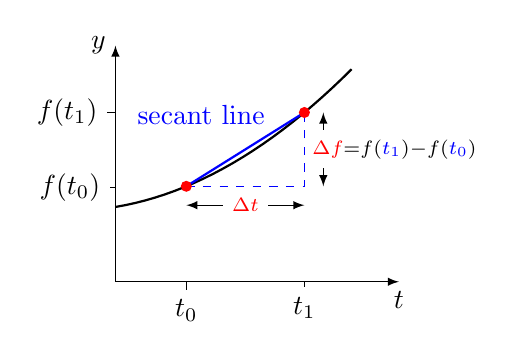
\begin{tikzpicture}[x=12mm,y=12mm,>=latex]
        \draw[black,->] (0,0) -- (3,0) node[below] {$t$};
        \draw[black,->] (0,0) -- (0,2.5) node[left] {$y$};
        % Ticks:
        \draw[thin,black] (0.75,0) -- (0.75,-3pt) node[below] {$t_0$};
        \draw[thin,black] (2,0) -- (2,-2pt) node[below] {$t_1$};
        \draw[thin,black] (0,1) -- (-2pt,1) node[left] {$f(t_0)$};
        \draw[thin,black] (0,{0.75+(2+1/2)^2/6}) -- (-3pt,{0.75+(2+1/2)^2/6}) node[left] {$f(t_1)$};
        \draw[black,thick] plot[domain=0:2.5] (\x,{0.75+(\x+1/2)^2/6});
      %
        \draw[thick,blue] (0.75,{0.75+(0.75+1/2)^2/6}) -- (2,{0.75+(2+1/2)^2/6}) node[near end,left,yshift=2mm] {secant line};
        \draw[thin,black,<->] (0.75,{0.75+(0.75+1/2)^2/6-0.2}) -- (2,{0.75+(0.75+1/2)^2/6-0.2}) node[midway,red,fill=white] {$\scriptstyle\Delta t$};
        \draw[thin,black,<->] (2.2,{0.75+(0.75+1/2)^2/6}) -- (2.2,{0.75+(2+1/2)^2/6}) node[midway,fill=white,right,xshift=-0.75em] {$\scriptstyle{\red\Delta f}=f({\blue t_1})-f({\blue t_0})$};
        \draw[thin,blue,dashed] (0.75,{0.75+(0.75+1/2)^2/6}) -- (2,{0.75+(0.75+1/2)^2/6}) -- (2,{0.75+(2+1/2)^2/6});
        % 
      %
        \fill[red] (0.75,{0.75+(0.75+1/2)^2/6}) circle (2pt);
        \fill[red] (2,{0.75+(2+1/2)^2/6}) circle (2pt);
    \end{tikzpicture}
  \end{minipage}
  \hfill
  \parbox{50mm}{%
    ${\red\Delta f}=$ change in $f$ \\
    ${\red\Delta t}=$ change in $t$\\[0.5em]
    \alert{Many ways to say same thing:}\\
    $\begin{array}{l}
       \left(\begin{array}{c} \text{{\blue average} rate of}\\ \text{change of $f$}\end{array}\right)  = \dfrac{\text{change in $f$}}{\text{change in $t$}}\\
       = \dfrac{\red \Delta f}{\red\Delta t}\\
       =  \text{slope of {\blue secant line}}
       = \dfrac{f({\blue t_1})-f({\blue t_0})}{{\blue t_1}-{\blue t_0}}
     \end{array}$
   }
   \pause

   The derivative is defined to be
   \begin{equation*}
     \lim_{\Delta t\to0} \left(\frac{\red\Delta f}{\red\Delta t}\right) 
     = \frac{df}{dt}
   \end{equation*}
   \pause

   Idea: As $t_1$ moves closer to $t_0$ the secant line approaches the {\blue tangent line}  at $t_0$.
   This is the line with the {\blue same slope} as the graph at $t_0$.

   % \fbox{{\red Let's watch a movie }} \qquad\qquad  No, not  {\blue The Bourne Identity}  :(\\

   % http://www.youtube.com/watch?v=AdQG2iSLDjA\\
   % http://www.youtube.com/watch?v=s3q8D79bjiE\&feature=related
}



\frame{
  \frametitle{Understanding Derivatives}

  There are many ways to {\blue think} about derivatives.  You {\blue
    need} to understand these to apply to problems. 
  \gap
  \gap 

  \begin{minipage}{0.35\linewidth}
    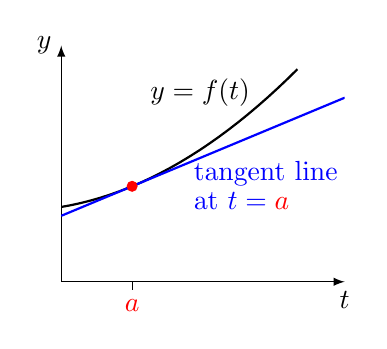
\begin{tikzpicture}[x=12mm,y=12mm,>=latex]
        \draw[black,->] (0,0) -- (3,0) node[below] {$t$};
        \draw[black,->] (0,0) -- (0,2.5) node[left] {$y$};
        % Ticks:
        \draw[thin,black] (0.75,0) -- (0.75,-3pt) node[below] {\red$a$};
        % \draw[thin,black] (2,0) -- (2,-2pt) node[below] {$t_1$};
        % \draw[thin,black] (0,1) -- (-2pt,1) node[left] {$f(t_0)$};
        % \draw[thin,black] (0,{0.75+(2+1/2)^2/6}) -- (-3pt,{0.75+(2+1/2)^2/6}) node[left] {$f(t_1)$};
        \draw[black,thick] plot[domain=0:2.5] (\x,{0.75+(\x+1/2)^2/6});
        \begin{scope}
          \clip (0,0) rectangle (3,2.5);
          \draw[blue,thick] plot[domain=0:3] (\x,{(0.75+1/2)*(\x-0.75)/3+0.75+(0.75+1/2)^2/6});
          \node[blue,right] at (1.3,1.15) {tangent line};
          \node[blue,right] at (1.3,0.85) {at $t={\red{}a}$};
          \node[left] at (2.1,2) {$y=f(t)$};
        \end{scope}
      %
      %
        \fill[red] (0.75,{0.75+(0.75+1/2)^2/6}) circle (2pt);
    \end{tikzpicture}
  \end{minipage}
  \hfill
  \parbox{60mm}{%
    slope of {\blue graph} at {\red a}\\
    = slope of {\blue tangent line} \\%\small{\red $\quad\quad^{discuss}$}\\
    = {\purple instantaneous rate of change} of $f$ at ${\red a}$\\
    \\
    $= \left(
      \begin{array}{l}
        \text{limit of average rate of change } \\ 
        \text{of $f$ over shorter and shorter}\\
        \text{ time intervals starting at\ {\red$a$}}
      \end{array}
    \right)$\\
    \\
    $=$ limit of slopes of secant lines\\
    $= f'({\red a})\ =\ \left. \dfrac{df}{dt}\right|_{t={\red a}}$
  }

}

\frame{
  \frametitle{Summary}

  \begin{itemize}
  \item[$\red \bullet$] How fast something changes $=$ {\blue rate of
      change}
    \bigskip

  \item[$\red \bullet$] {\red Instantaneous} {\blue rate of change} is
    the {\redgreen limit} of the average rate of change over shorter
    and shorter time spans. This gets around the ${\red 0/0}$
    problem. 
    \bigskip

  \item[$\red \bullet$] {\blue speed} $=$ rate of change of distance traveled.
    \bigskip

  \end{itemize}

}


\frame{
  \frametitle{Practical Meaning}

  Our goal is that you understand the {\blue practical meaning} of the
  derivative in various situations. 
  \gap
  \pause

  \begin{align*}
    f({\blue t})
    & = \text{temperature in ${}^{\circ}\ \text{F}$ at ${\blue t}$ hours after midnight}\\
    f({\blue 7})
    & = {\orange 48}\ 
      \text{means the temperature at {\blue 7}am was ${\orange 48}^\circ\ \text{F}$}\\
    f{\red '}({\blue 7})
    & ={\orange 3}\ 
      \text{means}\
      \text{at {\blue 7}am the temperature was rising at a rate of
      ${\orange 3}^{\circ}\ \text{F}/\text{hr}$} \\
    f{\red '}({\blue 9})
    & ={\orange -5}\ 
      \text{means}\ 
      \text{at {\blue 9}am the temperature was {\red falling} at a
      rate of ${\orange 5}^{\circ}\ \text{F}/\text{hr}$}\\ 
    & \hspace*{0.75in}\text{or {\red rising} at a rate of ${\orange
      -5}^{\circ}\ \text{F}/\text{hr}$}
  \end{align*}
  \gap
  \pause
  \begin{align*}
    g({\blue t})
    & = \text{distance from origin in cm of hamster on $x$-axis  after $\blue t$ seconds}\\
    g({\blue 7})
    & ={\orange 3}\
      \text{means after ${\blue 7}$ seconds hamster was ${\orange 3}$ cm from origin}\\
    g{\red '}({\blue 9})
    & ={\orange -5}\
    \text{means after {\blue 9} seconds our furry friend was running {\blue towards}}\\ 
    & \hspace*{0.25in}\text{the origin at a speed of ${\orange 5}\ \text{cm}/\text{sec}$}
  \end{align*}
}

\frame{
  \frametitle{Another Context}
  
  Suppose $f({\blue t})=$ temperature of oven in ${}^{\circ} \text{C}$
  after $t$ minutes.
  \smallskip

  What do $f(3)=20$ and $f{\red '}(3)=15$ mean?
  \begin{itemize}
  \item[A] After $20$ minutes the oven was at $3^{\circ}\ \text{C}$ and heating up at a rate of $15^{\circ}\ \text{C}/\text{min}$

  \item[B] After $3$ minutes oven temperature was $15^{\circ}\ \text{C}$ and cooling down at a rate to $20^{\circ}\ \text{C}/\text{min}$ 

  \item[C] The oven was heating up at rate of $3^{\circ}\ \text{C}/\text{min}$ after 15 minutes and also after 20 minutes

  \item[D] After 3 minutes the oven was at $20^{\circ}\ \text{C}$ and heating up at a rate of $15^{\circ}\ \text{C}/\text{min}$ 

  \item[E] None of the above

  \end{itemize}
  \pause
  \alert{Answer:}\ \fbox{D}

}

\frame{
  \frametitle{Yet Another Context}

  Now suppose $f(t)=$ the population of the ancient city of Lyrad in
  year $t$.  %{\blue C.E.} = {\blue C}urrent {\blue E}ra
  We are told that  $f(1550) = 1820$ and $f{\red '}(1650) = 1100$.
  Which of the following is true?

  \begin{itemize}
  \item[A] In 1550, the population was 1820 and rising at a rate of 1100 people per year

  \item[B] In 1650, the population was 1100 more than in 1550

  \item[C] In 1650, Lyrad contained 1100 people

  \item[D] In 1550, there were 1820 people in Lyrad, and by 1650 this had increased to 2920

  \item[E] None of above
  \end{itemize}
  \pause

  \alert{Answer:}\ \fbox{E}
}


\frame{
  \frametitle{Context: Mathematics}

  Suppose $f(0)=50$ and $f(10)=70$.  Which of the following is true?

  \begin{itemize}
  \item[A] For all $t$ between $0$ and $10$, the derivative is $f{\red'}(t)=2$

  \item[B] $f{\red'}(0)=2$

  \item[C] It is possible that $f{\red'}(0)=-8$

  \item[D] It is impossible that $f{\red'}(0)=-8$

  \item[E] None of above

  \end{itemize}
  \pause
  \alert{Answer:}\ \fbox{C}
  \gap 
  \pause

  We'll see later that, for example, that $f(x)=x^2-8x+50$ has $f(0)=50$,
  $f(10)=70$, and $f{\red '}(0)=-8$. 

}

\frame{
  \frametitle{Notice: No Time}

  \begin{minipage}{0.4\linewidth}
    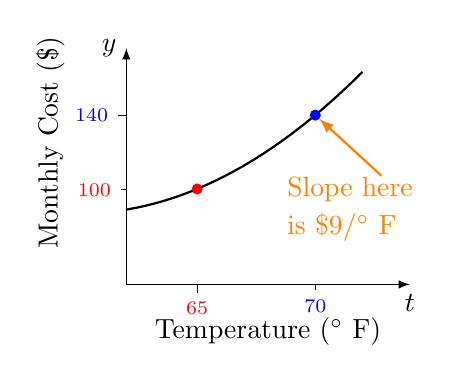
\begin{tikzpicture}[x=12mm,y=12mm,>=latex]
      \draw[black,->] (0,0) -- (3,0) node[below] {$t$};
      \draw[black,->] (0,0) -- (0,2.5) node[left] {$y$};
      % Ticks:
      \draw[thin,black] (0.75,0) -- (0.75,-3pt) node[below,red] {$\scriptstyle65$};
      \draw[thin,black] (2,0) -- (2,-2pt) node[below,blue] {$\scriptstyle70$};
      \draw[thin,black] (0,1) -- (-2pt,1) node[left,red] {$\scriptstyle100$};
      \draw[thin,black] (0,{0.75+(2+1/2)^2/6}) -- (-3pt,{0.75+(2+1/2)^2/6}) node[left,blue] {$\scriptstyle140$};
      \draw[black,thick] plot[domain=0:2.5] (\x,{0.75+(\x+1/2)^2/6});
      % 
      % \draw[thick,blue] (0.75,{0.75+(0.75+1/2)^2/6}) -- (2,{0.75+(2+1/2)^2/6}) node[near end,left,yshift=2mm] {secant line};
      % \draw[thin,black,<->] (0.75,{0.75+(0.75+1/2)^2/6-0.2}) -- (2,{0.75+(0.75+1/2)^2/6-0.2}) node[midway,red,fill=white] {$\scriptstyle\Delta t$};
      % \draw[thin,black,<->] (2.2,{0.75+(0.75+1/2)^2/6}) -- (2.2,{0.75+(2+1/2)^2/6}) node[midway,fill=white,right,xshift=-0.75em] {$\scriptstyle{\red\Delta f}=f({\blue t_1})-f({\blue t_0})$};
      % \draw[thin,blue,dashed] (0.75,{0.75+(0.75+1/2)^2/6}) -- (2,{0.75+(0.75+1/2)^2/6}) -- (2,{0.75+(2+1/2)^2/6});
      % 
      % 
      \fill[red] (0.75,{0.75+(0.75+1/2)^2/6}) circle (2pt);
      \fill[blue] (2,{0.75+(2+1/2)^2/6}) circle (2pt);
      \node[rotate=90] at (-0.8,1.5) {Monthly Cost (\$)};
      \node at (1.5,-0.5) {Temperature (${}^{\circ}\ \text{F}$)};
      \node[right,orange] at (1.6,1) {Slope here};
      \node[right,orange] at (1.6,0.6) {is $\$9/{}^{\circ}\ \text{F}$};
      \draw[thick,->,orange,shorten >=2pt] (2.7,1.15) -- (2,{0.75+(2+1/2)^2/6});
    \end{tikzpicture}
  \end{minipage}
  \hfill
  \begin{minipage}{55mm}
    $f(x) =$ monthly cost of heating house to $x^{\circ}\ \text{F}$
    \gap

    $f(70)=140$ means {\blue it costs \$140 to heat the house for one
      month to a temperature of $70^{\circ} \text{F}$.} 
    \pause
    \gap 

    ${\orange f'(70)=9}$ means {\blue {\red rate} at which cost increases
      as temperature changes is \$9 for each extra ${}^{\circ}\
      \text{F}$.}
  \end{minipage}
\pause
\gap 

In {\purple practical} terms this means {\blue you pay an extra \$9 during each month for each extra
$1^oF$}  . If you turn it up two degrees you pay an extra \$18 each
month. {\purple Each extra degree of warmth costs an extra \$9 each
  month.} 
In economics this is called a {\red marginal cost} or {\red marginal
  rate} \pause 
\gap 

This is not {\red exactly} true:\\  \qquad {\blue average} rate of
change versus {\blue instantaneous} rate of change.\\  In the
following examples we will ignore this subtlety. 


}


\frame{
  \frametitle{The Importance of Units}


  \begin{minipage}{0.4\linewidth}
    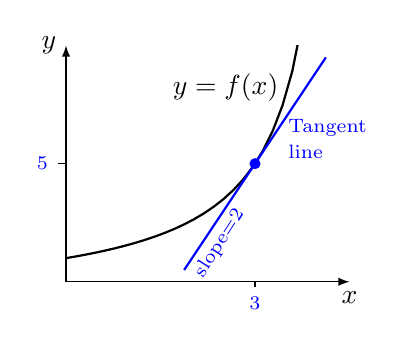
\begin{tikzpicture}[x=12mm,y=6mm,>=latex]
      \draw[black,->] (0,0) -- (3,0) node[below] {$x$};
      \draw[black,->] (0,0) -- (0,5) node[left] {$y$};
      % Ticks:
      \draw[thin,black] (2,0) -- (2,-2pt) node[below,blue] {$\scriptstyle3$};
      \draw[thin,black] (0,2.5) -- (-3pt,2.5) node[left,blue] {$\scriptstyle5$};
      \begin{scope}
        \clip (0,0) rectangle (3,5);
        \draw[black,thick] plot[domain=0:2.5] (\x,{-0.5-3/(\x-3)});
      \end{scope}
      \node[left] at (2.35,{-0.5-3/(2.35-3)}) {$y=f(x)$}; 
      \fill[blue] (2,{-0.5-3/(2-3)}) circle (2pt);
      % Tangent line to y=-0.5-3/(x-3), so y'=3/(x-3)^2 = 3 at x=2.
      % so through (2,2.5) with slope 3; y=3x-3.5
      \draw[thick,blue] (1.25,0.25) -- (2.75,4.75);
      \node[rotate=57.5,blue] at ({1.5+1*0.125},{1-1.5*0.125}) {$\scriptstyle\text{slope}=2$};
      \node[right,blue] at (2.25,3.25) {$\scriptstyle\text{Tangent}$};
      \node[right,blue] at (2.25,2.75) {$\scriptstyle\text{line}$};
    \end{tikzpicture}
  \end{minipage}
  \hfill
  \begin{minipage}{60mm}
    Told $f({\blue 3}) = 5$ and $f{\green '}({\blue 3})={\green 2}$
    \gap

    This means the slope of the tangent line to the graph $y=f(x)$ at $x=3$ is $2$.
    \gap 

    The derivative is this slope, so\ldots
    \gap 

    \fbox{The {\blue units}\ of $\dfrac{dy}{dx}$\ are $\dfrac{\text{units of y}}{\text{units of x}}$}
  \end{minipage}
  \bigskip
  \pause

  Heating example: derivative units are $\$/{}^{\circ}\ \text{F} = \text{dollars per degree F}$
  % Adrenaline example $bpm/mg =$\quad beats per minute per mg of adrenaline.\\
  \gap

  Units help you understand the {\blue meaning} of the derivative.

}

\frame{
  \frametitle{Get Pumped!}

  Adrenaline cause the heart to speed up.\\
  ${\blue x}=$ {\blue number of mg} (milligrams) of adrenaline in the blood.\\
  $f({\blue x})=$ {\orange number of beats per minute} (bpm) of the heart
  with ${\blue x}$ mg of adrenaline in the blood. 
  \gap

  What does $f{\red '}({\blue 5})={\orange 2}$ mean?
  \hfill\uncover<2->{\alert{Answer:}\ \fbox{E}}
  \begin{itemize}
  \item[A] When there are {\blue 5} mg of adrenaline the heart beats
    at {\orange 2} pbm

  \item[B] When the amount of adrenaline is increased by {\orange 2} mg
    the heart speeds up by {\blue 5} bpm

  \item[C] When the heart beats at {\blue 5} bpm the adrenaline is
    increased by {\orange 2} mg
 
  \item[D] When there are {\blue 5} mg of adrenaline the heart speeds
    up by {\orange 2}bpm
    
  \item[E] When there are {\blue 5} mg of adrenaline in the blood the
    heart speeds up by {\orange 2} bpm for each extra mg of adrenaline. 

  \end{itemize}
  \gap
  \textbf{Hint:}\ The {\purple units} of $ f{\red'}({\blue 5})$ are {\purple bpm per milligram of adrenaline}

}


\end{document}
